\documentclass{article}
\usepackage[portuguese]{babel}
\usepackage[utf8]{inputenc}

\usepackage{url}
\usepackage{alltt}
\usepackage{listings}
\usepackage{fancyvrb}
\usepackage{graphicx}
\usepackage{algorithmic}
\usepackage{hyperref}
\usepackage{listings}
\usepackage{xcolor}


\usepackage[lined,algonl,boxed]{algorithm2e}

\parindent=0pt
\parskip=2pt



\title {\textbf{Compiladores}\\\textbf{Licenciatura em Engenharia Informática} \\ \vspace{1cm}Anuário de Medicamentos}
\author{Daniel Oliveira - al74575 \\ Pedro Oliveira - al73346 \\ Francisco Gouveia - al74044 \\ Hugo Ribeiro - al73166 }
\date{\textbf{5 de Fevereiro de 2022}}



\begin{document}
\definecolor{mGreen}{rgb}{0,0.6,0}
\definecolor{mGray}{rgb}{0.5,0.5,0.5}
\definecolor{mPurple}{rgb}{0.58,0,0.82}
\definecolor{backgroundColour}{rgb}{0.94, 0.97, 1.0}

\lstdefinestyle{CStyle}{
    backgroundcolor=\color{backgroundColour},   
    commentstyle=\color{mGreen},
    keywordstyle=\color{magenta},
    numberstyle=\tiny\color{mGray},
    stringstyle=\color{mPurple},
    basicstyle=\footnotesize,
    breakatwhitespace=false,         
    breaklines=true,                 
    captionpos=b,                    
    keepspaces=true,                 
    numbers=left,                    
    numbersep=5pt,                  
    showspaces=false,                
    showstringspaces=false,
    showtabs=false,                  
    tabsize=2,
    language=C
}



\maketitle

\begin{picture}(10, 10)(-219, -300)

\includegraphics[scale=0.3]{utad.png}
\end{picture}


\vspace*{3cm}
\begin{abstract}
\centering
\par No âmbito da Unidade Curricular de Compiladores, foi-nos pedido pela docente da cadeira, que implementássemos, em grupo, um Sistema de Consulta de Medicamentos, que fosse acessível a qualquer farmácia através de um \emph{Browser HTML}.
\par É imprescindível o conhecimentos de várias ferramentas como o \emph{Lex} e o \emph{Yacc}, de modo a gerar a partir destes um reconhecedor léxico e sintáctico respetivamente. Também é indispensável a programação em C e, por último, mas não menos importante, o conhecimento da escrita em \emph{LaTeX} para o desenvolvimento do relatório presente.

\end{abstract}

\thispagestyle{empty}

\pagebreak


\vspace*{2cm} \Large\tableofcontents \vspace*{\fill}
\thispagestyle{empty}
\setcounter{page}{0}
\pagebreak

\vspace{1cm}
\large\section{Introdução}

\hspace*{1.5em}Na âmbito da Unidade Curricular de Compiladores dirigida pela professora Teresa Perdicoúlis foi nos proposto a elaboração de um Sistema de Consulta de medicamentos, para auxiliar o Instituto Farmacêutico do Ministêrio da Saúde na gestão de medicamentos brancos. Este teria que, eventualmente, ser acessível a qualquer farmácia através de um \emph{Browser HTML}. Para isto, foi realizado um Analisador Sintático, e um Analisador Léxico, que é capaz de analisar o ficheiro de texto, com a formatação correta, de forma a colocar em diferentes categorias, os diferentes medicamentos. Depois disto também foi desenvolvida a respetiva gramática, analisando se o ficheiro de texto teria as respetivas propriedades expostas de forma correta. 
\par \hspace*{1.5em}Podemos demarcar uma estrutura para este relatório da seguinte forma: um resumo Inicial, onde colocamos os principais pontos a ser abordados, dois capítulos que se referem a Análise, e Testes do \textit{Software} implementado. A Análise aborda temas teóricos que são essenciais para a compreensão dos assuntos aqui debatidos, e, por último, os Testes referem-se ao trabalho da equipa, de forma prática, ao testar o \emph{Software} desenvolvido, observando atentamente o seu comportamento. Em último lugar temos a Conclusão, que vai demonstrar e explicar os resultados obtidos, com uma análise \emph{a posteriori}. Adicionalmente, colocamos dois Apêndices, um referente à descrição da equipa responsável pelo trabalho, e as suas diferentes funções, e em segundo lugar, um para o Anexo dos \emph{Source Files}.



\par \hspace*{1.5em}Em termos do Sistema Operativo usado, utilizamos o \emph{Manjaro KDE} (uma distribuição do \emph{Linux}, com base em \emph{Arch}), e o leitor de ficheiros \emph{KATE} nativo para o Sistema Operativo respetivo, para desenvolver tanto o AL, Analisador Léxico, como o Analisador Sintático, AS. Inicialmente desenvolvemos o AL, escrito em LeX, de modo a que este reconhecesse símbolos terminais e tokens. Seguidamente desenvolvemos o analisador sintático, que por sua vez foi escrito em Yacc, que recebe os símbolos recebidos do AL, e as suas \emph{tokens} e verifica se a sequência em causa respeita as regras de derivação ou produções da gramática. 
\par \hspace*{1.5em}Para finalizar realizamos este relatório em LaTeX, onde anotamos toda a informação necessária à compreensão do projeto.

\pagebreak

\section{Análise}
\subsection{Descrição informal}
\hspace*{1.5em}O nosso grupo irá realizar este trabalho através de ferramentas lecionadas ao longo do semestre.
Iremos usar o \emph{Lex} (que é o exemplo mais divulgado de ferramentas de geração de analisadores léxicos), para fazer o reconhecimento dos \emph{tokens} necessários ao problema descrito.
Também iremos usar o Yacc (que é o exemplo mais divulgado de ferramentas de geração de analisadores sintáticos), para gerar um reconhecedor e implementar toda a parte dois do problema descrito.
Por último mas não menos importante, também usamos a programação em C para realizar testes.

\vspace{10cm}

\section{Testes}
\subsection{Alternativas e Problemas de Implementação}

\hspace*{1.5em}Na realização do projeto tivemos dificuldades em desenvolver, em ambos os analisadores, a sua implementação em C. Adicionalmente, na secção do Analisador Sintático tivemos uma dificuldade mais geral, na formulação e aplicação da gramática do mesmo, conseguindo porventura, gerar a \emph{parsing table} com sucesso, como iremos ver mais à frente.


\subsection{Testes Realizados e Resultados}
\newcommand{\keyword}[1]{\textbf{#1}}
\newcommand{\tabhead}[1]{\textbf{#1}}
\newcommand{\code}[1]{\texttt{#1}}
\newcommand{\file}[1]{\texttt{\bfseries#1}}
\newcommand{\option}[1]{\texttt{\itshape#1}}

\large\textbf{Primeiro Teste: \emph{medicamentos.txt}}
\begin{lstlisting}[style=CStyle]
Symposium: 2021
		[Analgesico,Antibiotico]
		[
		 (Moment,1,Analgesico,Paracetamol,4.5,{Roche},{Qualquer-Bial});

		(Antigripine,2,Antibiotico,Acetalilico,6.,{Fabt,Faba},{Aga-Fabc,Agb-Fabh})  
		]
    
\end{lstlisting}
\par
\normalsize\textbf{Resultado: \emph{saida1.txt}}

\begin{lstlisting}[style=CStyle]
Times: 1 | Found SYMPOSIUM: Symposium
Times: 1 | Found Signals: :
Times: 1 | Found Spaces
Times: 1 | Found Year: 2021
Times: 2 | Found Spaces
Times: 3 | Found Spaces
Times: 4 | Found Spaces
Times: 2 | Found Signals: [
Times: 1 | Found ID: Analgesico
Times: 3 | Found Signals: ,
Times: 2 | Found ID: Antibiotico
Times: 4 | Found Signals: ]

[...]

PARSING SUCCESS!

\end{lstlisting}

\large\textbf{Segundo Teste: \emph{medicamentosGood.txt}}
\begin{lstlisting}[style=CStyle]
Symposium: 2022
		[Analgesico,Antibiotico]
		[
		 /- Medicamento 1 -/
		(Moment,1,Analgesico,Paracetamol,4.5,{Roche},{Qualquer-Bial});

		 /- Medicamento 2 -/
		(Antigripine,2,Antibiotico,Acetalilico,6.,{Fabt,Faba},{Aga-Fabc,Agb-Fabh})
		]



\end{lstlisting}

\normalsize\textbf{Resultado: \emph{saida2.txt}}

\begin{lstlisting}[style=CStyle]
Times: 1 | Found SYMPOSIUM: Symposium
Times: 1 | Found Signals: :
Times: 1 | Found Spaces
Times: 1 | Found Year: 2022
Times: 2 | Found Spaces
Times: 3 | Found Spaces
Times: 4 | Found Spaces
Times: 2 | Found Signals: [
Times: 1 | Found ID: Analgesico
Times: 3 | Found Signals: ,
Times: 2 | Found ID: Antibiotico
Times: 4 | Found Signals: ]

[...]

PARSING SUCCESS!

\end{lstlisting}

\vspace{2cm}

\section{Conclusão}
\hspace*{1.5em}Apesar de algumas dificuldades na resolução deste projeto, após refletirmos sobre as mesmas, podemos admitir que fomos capazes de progredir no sentido de resolver os problemas que nos foram surgindo ao longo deste trabalho prático.
Em âmbito de conclusão, confessamos que, estamos cientes das limitações que o nosso trabalho apresenta, mas, não obstante da sua solidez em termos de erros, segurança, e praticidade. Admitimos assim que, estamos satisfeitos e orgulhosos da nossa evolução ao longo da realização do relatório, atingindo assim grande parte dos objetivos propostos.


\pagebreak


\appendix
\section{Source Files}
\large\textbf{Analisador Léxico}

\vspace{2cm}


\begin{figure}[!h]
\centering
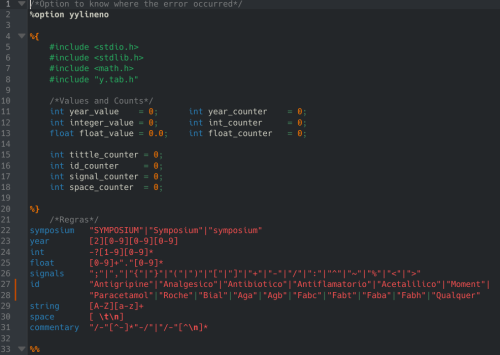
\includegraphics[width=0.7\textwidth]{AL1.png}
\end{figure}

\begin{figure}[!h]
\centering
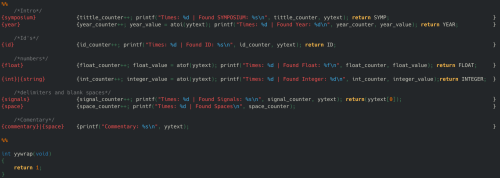
\includegraphics[width=1\textwidth]{AL2.png}
\end{figure}

\begin{figure}[!h]
\centering
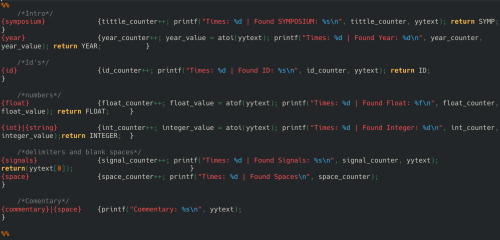
\includegraphics[width=1\textwidth]{AL3.png}
\end{figure}

\pagebreak

\large\textbf{Analisador Sintático}



\begin{figure}[!h]
\centering
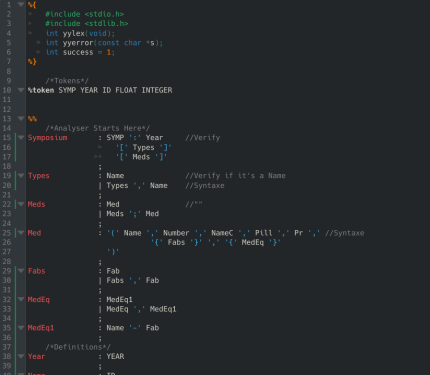
\includegraphics[width=0.8\textwidth]{AS1.png}
\end{figure}

\begin{figure}[!h]
\centering
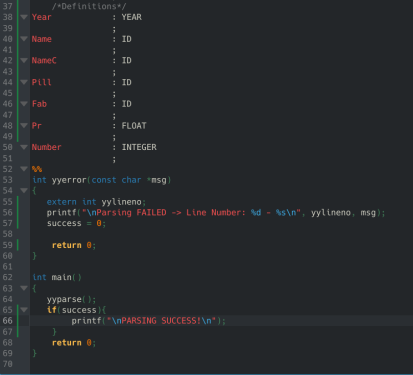
\includegraphics[width=0.8\textwidth]{AS2.png}
\end{figure}



\pagebreak



\vspace*{2cm}\section{Equipa}
Este projeto foi realizado por um grupo de 4 elementos:\\
\par Daniel Oliveira, Pedro Oliveira e Hugo Ribeiro foram os responsáveis pelo relatório. Francisco Gouveia foi o responsável pelo AL nas diferentes linguagens assim como o AS.
\vspace*{\fill}



\end{document}
